\section{Core Architecture}

\subsection{VLIW Architecture}

The \KalrayK core implements a 64-bit 8-issue Very Long Instruction
Word (VLIW) architecture with a 8-stage instruction pipeline. Groups of
instructions that issue together are identified and encoded by the assembler into
\emph{instruction bundles} (or ``bundles''). Inside a bundle, the source registers of all instructions are read before any target register is written. This key feature of VLIW execution enables to swap two registers by bundling two copy instructions that target each other source register. In also enables to expose wider SIMD instructions that what the ISA proposes by bundling them.

Compared to traditional VLIW architectures, whether Fisher-style or EPIC-style, the distinguishing features of the \KalrayK architecture are:
\begin{itemize}
    \item No need for inserting NOP instructions to complete bundles (horizontal NOPs) or to satisfy register dependences (vertical NOPs).
    \item Individual instructions are 32-, 64- or 96-bit wide in order to inline the 32-bit or 64-bit immediate constant operands.
    \item The core appears as a in-order superscalar to the compiler, as any parallel instruction group identified by instruction scheduling can be encoded in a bundle.
    \item Support of predication and masking for any non-control instruction without the cost and complexity of a fully predicated ISA by bundling dedicated control unit instructions.
\end{itemize}

The \KalrayK core architecture has 64$\times$64-bit general-purpose registers (GPRs) that
contain boolean, integer, address, fixed-point and floating-point data types. The core supports the corresponding arithmetic instructions and also their SIMD versions on 128-bit data held into register pairs.
The \KalrayK core architecture is byte-addressable little endian. The architecture is also
a bit-little endian, meaning that bit 0 of any data is always the least significant bit
(little endian), and is shown at the rightmost position in figures.

The \KalrayK core architecture supports an optional coprocessor extension (historically called TCA) which is tightly integrated into the instruction pipeline. This coprocessor extension hosts a 32$\times$512-bit register file is aiming at accelerating compute intensive applications using 512-bit SIMD arithmetic. The coprocessor extension itself can be further connected to external compute resources to expand the core capabilities.

\subsection{Data Types and Representations}

The \KalrayK core instruction set architecture (ISA) efficiently supports 8-bit,
16-bit, 32-bit, 64-bit, and 128-bit scalar types, and also 8-bit, 16-bit, 32-bit or 64-bit data
types packed into 128-bit containers. The non-packed data types are interpreted as
signed integers, unsigned integers, and IEEE~764 binary floating-point numbers.

\subsubsection{Signed Integers}

An integer is expressed as a binary number of 2's complement and is 8-, 16-,
32-, 64-bit, or 128-bit long. Regardless of its length, the bit 0 of an integer
is always the least significant bit. Because 2's complement is used, the most
significant bit is used as a sign bit.

\begin{center}
\begin{tabular}{|c|c|} \hline
{Data Length} & {Value Range} \\ \hline
{8 bits} & $-2^7$ to $+2^7 - 1$ \\
{16 bits} & $-2^{15}$ to $+2^{15} - 1$ \\
{32 bits} & $-2^{31}$ to $+2^{31} - 1$ \\
{64 bits} & $-2^{63}$ to $+2^{63} - 1$ \\
{128 bits} & $-2^{127}$ to $+2^{127} - 1$ \\ \hline
\end{tabular}
\end{center}

\subsubsection{Unsigned Integers}

An unsigned integer is a binary number whose most significant bit has a positive
weight and is 8-bit, 16-bit, 32-bit, 64-bit, or 128-bit long.

\begin{center}
\begin{tabular}{|c|c|} \hline
{Data Length} & {Value Range} \\ \hline
{8 bits} & $0$ to $+2^8 - 1$ \\
{16 bits} & $0$ to $+2^{16} - 1$ \\
{32 bits} & $0$ to $+2^{32} - 1$ \\
{64 bits} & $0$ to $+2^{64} - 1$ \\
{128 bits} & $0$ to $+2^{128} - 1$ \\ \hline
\end{tabular}
\end{center}

\subsubsection{Floating-Point Numbers}

The \KalrayK core represents floating-point numbers in little-endian binary
format, according to the IEEE754~2008 standard.

For 16-bit binary floating-point numbers, the representation is as follows:

\bitfields{ 1/s, 5/exponent, 10/fraction}

For 32-bit binary floating-point numbers, the representation is as follows:

\bitfields{ 1/s, 8/exponent, 23/fraction}

For 64-bit binary floating-point numbers, the representation is as follows:

\bitfields{ 1/s, 11/exponent, 20/fraction, 32/fraction}

\subsubsection{Load and Store Instructions}

Load and stores transfer data between between the general purpose registers of the core and addressable memory. Data transfers width is any of 8, 16, 32, 64, 128, or 256 bits:
\begin{itemize}

\item Loading 8-bit, 16-bit and 32-bit from memory produces a 64-bit word by either sign-extending or zero-extending the loaded value.

\item When loading 64-bit data, they are directly stored into the target
  register.

\item When loading 128-bit data, they are directly stored into the target
 register pair ($R_{i}$ and $R_{i+1}$, with $i$ even).

\item When loading 256-bit data, they are directly stored into the target
 register quadruple ($R_{i}$ to $R_{i+3}$, with $i$ multiple of 4).

\end{itemize}


\subsection{VLIW Instruction Bundles}

\subsubsection{Instruction Bundle Composition}

The \KalrayK instruction bundle is composed of 32-bit instruction syllables. Instruction syllables in a bundle encode up to two BCU (Branch \& Control Unit) instructions, two ALU (Arithmetic \& Logic) instructions, two LSU (Load-Store Unit) instructions, two EXT (coprocessor Extension) instructions, and up to eight IMMX (Immediate Extension).
For each syllable: \begin{itemize}
\item Bit 31 is the Parallel bit: 0 if syllable is last in the bundle, else 1.
\item Bits 30 and 29 encode the Steering: 0 for BCU; 1 for LSU; 2 for ALU; and 3 for EXT.
\item Immediate extension (IMMX) syllables have Steering 0 and provide 27 bits of payload.
\item An IMMX  syllable specifies its target with a 2-bit Tag encoded in bits 28 and 27.
\end{itemize}

The \KalrayK architecture provides issue slots called BCU0, BCU1, ALU0, ALU1, LSU0, LSU1, EXT0, EXT1 that correspond to execution units (EXUs).
\begin{itemize}
\item The IMMX syllable Tag specifies its target issue slot as: 0 for ALU0; 1 for ALU1, 2 for LSU0; 3 for LSU1.
\item One or two IMMX syllables may apply to any of the ALU or LSU instructions.
\item A BCU instruction may also benefit from a branch offset extension by positioning a syllable with Steering = 0 and Tag = 0 next to it.
\item Instructions executed on the EXT EXUs may not receive an immediate extension.
\item The maximum number of syllables in an instruction bundle is 18, but the number accepted in a valid bundle is set to 16.
\end{itemize}

Instructions that are PC-relative are based on the PC of their first syllable in the bundle.

\subsubsection{Operand Immediate Extensions}

The core subset of 64-bit integer instructions and load/store instructions may encode a signed 10-bit immediate operand. With one IMMX syllable, a 37-bit signed immediate operand is available. With two IMMX syllables, a 64-bit immediate operand is available. Moreover, instructions called MAKE may encode a 16-bit signed immediate in a single syllable:

\begin{center}
\begin{tabular}{|l|l|l|} \hline
Instruction Type & Immediate Constant & Instruction Size \\ \hline
MAKE & 16 bits signed & 32 bits \\
MAKE & 37 bits signed & 64 bits \\
MAKE & 64 bits & 96 bits \\
ALU, LSU & 10 bits signed & 32 bits \\
ALU, LSU & 37 bits signed & 64 bits \\
ALU, LSU & 64 bits & 96 bits \\ \hline
ALU & 32 bits signed & 64 bits \\
SIMD & 32-bit splatted & 64 bits \\
\hline \end{tabular}
\end{center}

In this table, the two last rows correspond to the so-called "magic immediate" extensions. In this case, the base instruction does not have a 10-bit signed immediate operand that could be extended. Rather, its source operands are GPRs specified by a 6-bit field. When an IMMX syllable targets such an instruction, the 6-bit register specifier is interpreted a one 'splat' bit and 5 payload bits. The 5 payload bits and the IMMX 27-bit payload provide 32 bits. These 32 bits are either sign-extended, or the 32 bits are replicated to the operand width. The latter is useful to provide immediate operands to SIMD instructions with up to 32-bit wide lanes.

\subsubsection{Instruction Bundle Binary Layout}

Instructions in a bundle are dispatched to the \KalrayK issue slots in the order BCU0, BCU1, ALU0, ALU1, LSU0, LSU1, EXT0, EXT1. So the first syllable of any instruction must follow this order in the bundle binary layout. The immediate extension syllables (Steering = 0) for ALU and LSU instructions must appear last in the bundle with the least significant bits of payload first in case of instructions with two IMMX syllables. In case of a BCU instruction with extended offset, its IMMX appears as the second syllable (the first being the branch instruction).

Moreover, instructions dispatch starts by the EXUs that have the most capabilities: \begin{itemize}
\item BCU0 may execute all BCU instructions, while BCU1 only accepts BCU instructions that may dual issue.
\item ALU0 may execute all ALU FULL instructions and ALU1 may execute all ALU LITE instructions. LSU0 and LSU1 may execute the ALU TINY instructions.
\item LSU0 may execute all the LSU instructions, while LSU1 only accepts the load and DTOUCHL instructions.
\item EXT0 may execute the COMP instructions, and EXT1 the MISC instructions.
\end{itemize}

\smallskip
%{\color{red}Please refer to Section~\ref{sec:encoding} for the details of instruction bundle encoding.}

\subsubsection{Instruction Bundles in Assembly Language}

At the assembly language level, instructions may appear in any order (except for branch instruction that are ordered) and the immediate operand extensions are not apparent. These extensions are inferred from the number of bits required to encode the immediate values.

Each assembler instruction is separated from the next one either by an end of line or by a `\texttt{;}' character. The end of the bundle is marked by a `\texttt{;;}' alone in its line. Like with most assembly languages, a single `\texttt{\#}' character introduces a comment that extends until the end of line.

At the assembly language level, the control instructions that drive instruction predication or masking of other (non-control) instructions in the bundle do not appear explicitly. Rather, the assembler collects the prefix syntax of the predicated or masked instructions, and consolidate them as separate control unit instructions in the bundle binary encoding.

\section{Core Implementation}

\subsection{Datapath Organization}

\subsubsection{Execution Units and Register Files}

The \KalrayK core includes two main arithmetic, logic and floating-point units that include
multiply-accumulate instructions (ALUs), two load/store units (LSUs) and two branch/control unit (BCUs).
These six execution units are primarily connected through the GPR register file, that supports
reading up to eleven 64-bit registers plus two 256-bit register quadruples, and writing up to
one 64-bit register, two 128-bit register pairs and two 256-bit register quadruples per clock
cycle. The six execution units also share system function registers (SFRs) for program control
and compute status (Figure~\ref{fig:dolomites-vliwcore}).


\begin{figure}
\centering
  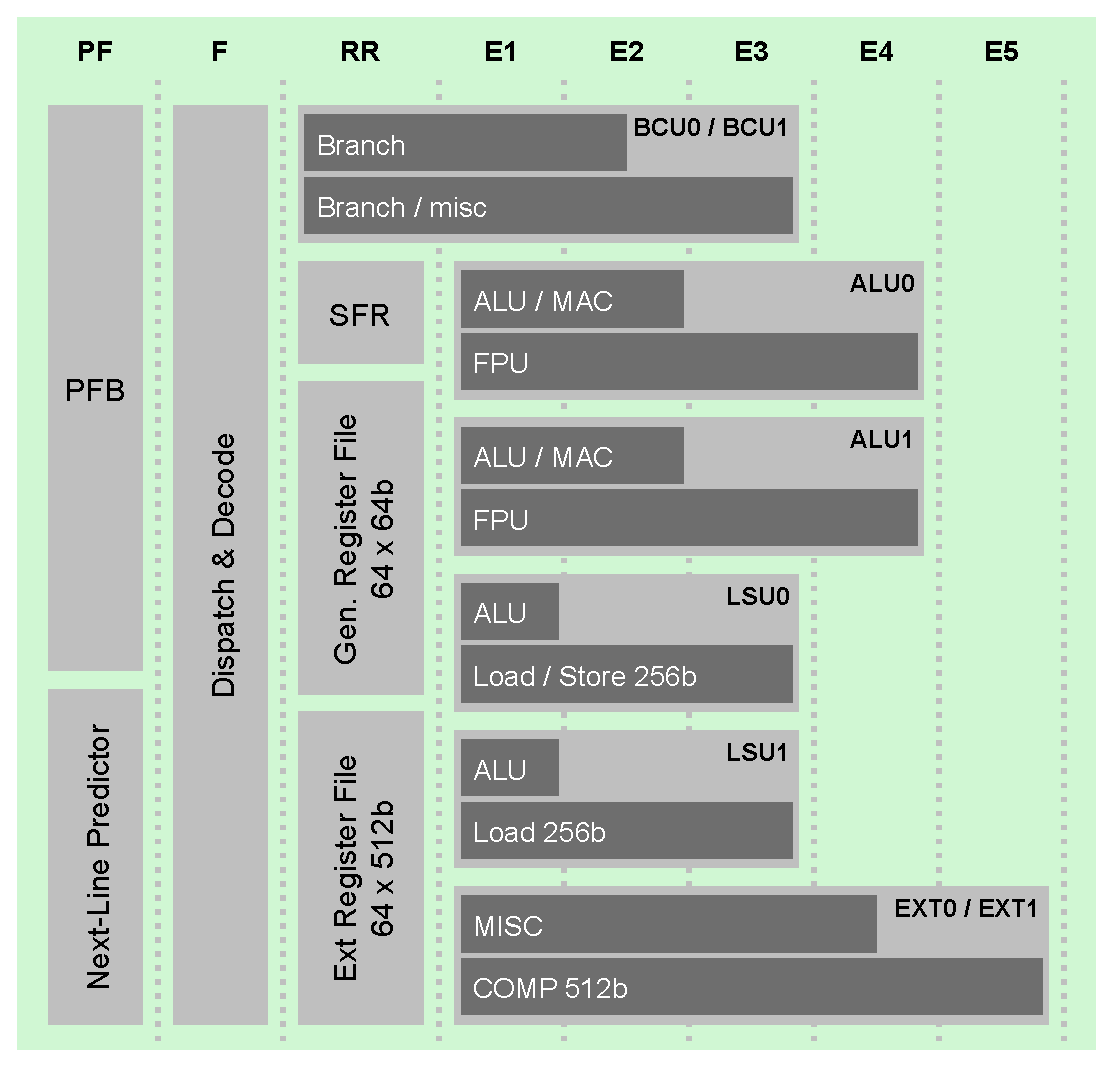
\includegraphics[width=.5\textwidth]{dolomites-vliwcore}
\caption{\KalrayK VLIW core block diagram.}
\label{fig:dolomites-vliwcore}
\end{figure}


\subsubsection{Instruction Pipeline Stages}

The instruction pipeline is composed of a Prefetch (PF) stage, a Fetch stage (F) and a Register
Read (RR) stage, followed by five execution stages: E1, E2, E3, E4, and E5 (coprocessor extension).
All executions begin in E1, with the exception of branches that are computed and taken as soon as
resolved by the branch predictor at ID or RR stage. Most operands are read or bypassed for 
execution at the end of RR. This pipeline allows arithmetic and load/store
instructions to execute for up to four cycles if needed. The results of instructions that
complete earlier than E4 are made available for bypassing as operands to subsequent instructions.

The instruction pipeline of the \KalrayK core is interlocked, i.e., run-time
stalls occur whenever an instruction tries to access a register that is not
data-ready.


\subsubsection{Prefetch Buffer (PFB)}

The Prefetch Buffer (PFB) is in charge of fetching instruction bundles and
preparing instructions for dispatch to the execution units.
The PFB manages 4 lines of 8$\times$32-bit and
receives blocks of 8$\times$32-bit from the instruction cache every clock cycle,
assuming that these blocks are in the instruction cache (fetch hit) and do not
cross a level-1 cache line boundary (64-byte).

The PFB attempts to fetch ahead in order to keep its 4 lines of 8$\times$32-bit
full. When a branch is taken, the PFB is flushed and a new fetch starts from the
target address. After a branch, the PFB takes one cycle to fetch the next bundle
from the cache. Branching to a bundle that is split over two cache lines
requires two cycles to fetch the bundle.

The PFB also provides 0-cycle overhead hardware loop support, allowing to
automatically jump from the end to the beginning of a hardware loop without
branch penalty.

\subsubsection{Branch and Control Unit (BCU)}

The \KalrayK core has two branch and control units (BCUs).
These units support PC-relative and indirect branches or calls. One branch unit also supports
hardware looping, also known as zero overhead loops.
Due to instruction pipelining, all taken branches (not including hardware looping) involve
run-time stalls: one cycle for unconditional direct branches and two cycles for
conditional and indirect branches. Not taken conditional branches involve no
stalls. Branch stalls are not visible at the architecture level, that is, there
are no delayed branches.
Up to two conditional branches, or one conditional branch and one unconditional branch (including function call/return), or one branch with extended offset, can be bundled with non-control instructions.
Branches within a bundle are ordered, so the first branch resolved as taken effectively branches ignoring the second one, even if the latter resolves as taken.

The BCU also supports predication and masking of other instructions in the bundle:
\begin{itemize}
    \item Predication allows a subset of instructions in the bundle to be conditionally disabled, depending on a predicate evaluated in one of the two BCUs. Predication is achieved by executing a GUARD instruction, which evaluates the same condition as the conditional branch instruction CB, but whose last operand is a 8-bit mask where each bit specifies the execution unit (ALU0, ALU1, LSU0, LSU1, EXT0, EXT1, ...) to be predicated.

    \item Similarly, the output of data processing instructions can be masked at the granularity of a 8-bit, 16-bit, 32-bit, 64-bit SIMD lane by executing a BLEND instruction, which specifies its target execution units with the same 8-bit mask as GUARD. The BLEND instruction reads a source operand where each bit corresponds to a SIMD lane, with the byte size of the lane provided by a modifier, and the masked instructions only write the active lanes.
\end{itemize}

In case of clusters composed of several processing elements (PE), each \KalrayK PE core is connected to its direct predecessor and successor by wires that transport events for direct
synchronization. The BCUs executes all instructions related to waiting and signaling events.

\smallskip 
%{\color{red}See Section~\ref{sec:BCU-instructions} for BCU instructions.}

\subsubsection{Arithmetic and Logic Units (ALUs)}

The \KalrayK core has two main arithmetic and logic units (ALU0 and ALU1). These units operate on both integer and floating-point values.

\paragraph{ALU Integer Operations}
Each arithmetic and logic unit (ALU) is capable of executing one instruction per cycle on 64-bit integers or on 128-bit SIMD integer data. Integer signed, unsigned, and signed saturated instructions are available on each ALU. The results of the ALUs are 64-bit or 128-bit wide and can be used as operands of the next instruction bundle (one clockycle latency), except for multiplication- and division-related instructions. In addition, the ALUs are capable of executing specific instructions such as building immediate values up to 64 bits (MAKE), adding constants to the instruction PC (PCREL), inserting/extracting bit-fields from 64-bit words, and moving data from/to the coprocessor extension.

\smallskip 
%{\color{red}See Section~\ref{sec:ALU-instructions} for integer instructions.}

\paragraph{ALU Floating-Point Operations}

The \KalrayK core ALUs perform floating-point operations on 16-bit (binary16 or FP16), 32-bit (binary32 or FP32) and 64-bit (binary64 or FP64) IEEE~754 floating-point formats and include addition, multiplication, multiply-add, comparisons and conversion from/to integer formats. All IEEE~754 standard rounding modes are supported, with the addition of the round-to-odd mode. All FPU operations correctly operate on the subnormal values. The only deviation from the IEEE~754 standard is that a canonical NaN is produced if any input or the result on an operation is a NaN.

The \KalrayK core ALUs include a dual multiply-add unit (FMA) in
single precision and a multiply-add unit in double precision. All floating-point
instructions operate in conformance with the IEEE~754-2008 standard for binary
floating-point numbers, including sub-normals and four rounding modes. Correctly
rounded division and square root instructions are available by executing
Newton-Raphson iterations on values provided by seed generators for the 32-bit
and 64-bit floating-point $\frac{1}{x}$ and $\frac{1}{\sqrt{x}}$.

\smallskip
%{\color{red}See Section~\ref{sec:FPU-instructions} for Floating-point instructions.}

\subsubsection{Load/Store Units (LSU)}

The \KalrayK core has a two load/store units (LSUs); they are fully pipelined with a latency of three cycles in the data cache. These units can take up to three operands (two 64-bits operands for the effective base+offset address computation, and one up to 256-bits for the stored data).
At every clock cycle, the core is able to do two loads of 256, 128 or 64 bits to registers
(simple, double or quadruple) or one load and one store of 256, 128 or 64 bits to/from registers
(simple, double or quadruple). When reading less than 64 bits from memory, load instructions zero-extend or sign-extend the memory datum to the 64 bits of the destination register.
Loads and stores are also available to the coprocessor EXT with data widths of 256 bits. \medskip

The LSU also supports atomic memory operations in various data sizes:

\begin{tabular}{|c|c|c|} \hline
{basic operation} & {logic operations} & {supported sizes} \\ \hline
load  & add, set, xor, clear, saturating decr & 1B, 2B, 4B, 8B \\
store & add, set, xor, clear & 1B, 2B, 4B, 8B \\
swap  & -                    & 1B, 2B, 4B, 8B \\
compare and swap (valued)  & - & 1B, 2B, 4B, 8B, 16B  \\
compare and swap (boolean) & - & 1B, 2B, 4B, 8B, 16B  \\ \hline
\end{tabular} \medskip

The \KalrayK core supports the following addressing modes for regular memory accesses:
\begin{itemize}
\item A base register plus a 10-bit signed, unscaled immediate constant.
\item A base register plus a 37-bit signed, unscaled immediate constant.
\item A base register plus a 64-bit signed, unscaled immediate constant.
\item A base register plus or minus an index register.
\end{itemize}

The \KalrayK core supports the following addressing modes for atomic memory accesses:
\begin{itemize}
\item A base register only.
\item A base register plus a 27-bit signed, unscaled immediate constant.
\end{itemize}

In non-device memory areas, the \KalrayK core supports memory accesses with
misaligned effective addresses for regular loads/stores.  Atomic instructions
and accesses to device memory areas must be aligned on the size of the accessed
object. If not, the \KalrayK core will take a DMISALIGN trap.

In order to speed up integer intensive applications, each LSU also includes a 64-bit
light ALU unit that execute a subset of the 64-bit arithmetic and logic instructions.
This light ALU can be used if the corresponding LSU is not used for memory access
instructions in the same bundle.

\smallskip
%{\color{red}See Section~\ref{sec:LSU-instructions} for LSU instructions.}


\subsubsection{Instruction Scheduling Constraints}

In addition to the bundle structure, which is defined at the architecture level, instruction scheduling is further constrained by micro-architecture resource and latency constraints. In particular, the Write-After-Read (WAR) dependence latency is zero, the Write-After-Write (WAW)
latency is one, and the Read-After-Write (RAW) dependence latency is strictly positive.

%{\color{red}\smallskip Please refer to Section~\ref{sec:constraints} for detailed instruction bundling constraints.}

The \KalrayK core scheduled resources abstract the hardware resources shared by instructions simultaneously issued on different execution units. These resources correspond to the register file access ports that are not dedicated to a particular execution unit (Figure~\ref{fig:regfile-kv4}): \begin{description}
\item[AUXR] LSU0 uses a 256-bit read port of the core registers at E1 to supply the stored values and execute read-modify-write atomic instructions.
\item[AUXW] Two 256-bit write ports of the core registers are used at E3, respectively, by LSU0 and LSU1 to receive the loaded values.
\item[MEMW] Ensures single issue of memory store and atomic instructions.
\item[SSFU] A 512-bit operand read port at RR of the MISC unit is shared with the SIMD SFU unit.
\item[ACCR] The 512-bit accumulator read port at E1 of the COMP unit is used by LSU0 to store extension register values (XSO instructions) and by the ALUs to get values from the extension registers (XMOVEF* instructions).
\item[OUTW] The 1024-bit output port at E2 of the MISC unit is used by the core to move values to the extension registers (XMOVET* instructions).
\end{description}

\begin{figure}
\centerline{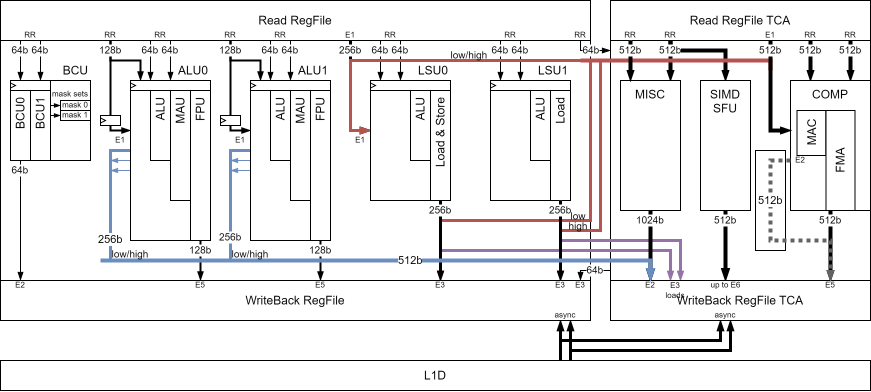
\includegraphics[width=1.25\columnwidth]{regfile-kv4}}
\caption{\KalrayK core register files accesses.}
\label{fig:regfile-kv4}
\end{figure}


\subsection{Memory Subsystem}


The \KalrayK core memory subsystem includes the following components: \begin{itemize}

\item Processor cache arbiter (PCA).
\item Instruction cache (IC).
\item Data cache (DC).

\end{itemize}

\subsubsection{Processor Cache Arbiter (PCA)}

The \KalrayK core features separate instruction and data caches that support,
respectively, the fetch of instructions and the load/store data accesses.
These two independent caches are connected to the outside memory system by a
round-robin arbiter: the PCA.

\subsubsection{Memory Management Unit (MMU)}

The \KalrayK core includes a memory management unit that performs address translation, ensures memory protection between processes and enforces memory caching and sharing policies. The MMU is described in detail in ~\ref{sec:memory-management-unit}

\subsubsection{Instruction Cache (IC)}

The instruction cache of the \KalrayK core receives fetch requests from the PFB
and returns groups of up to eight 32-bit syllables that will later be assembled
into bundles by the prefetch buffer. It has 32K bytes capacity, is 4-way set
associative with LRU (Least Recently Used) replacement policy and 64-byte
lines.

When the instruction words requested by the PFB are not in the cache, they are
fetched from the memory system (with a critical-word-first scheme) and stored
into the cache. During this time the core may stall, depending on the state of
the PFB. The requested syllables are then returned to the PFB.

To invalidate the instruction cache safely, the core must execute the IINVAL
instruction followed by the BARRIER instruction. This will invalidate the whole
instruction cache, and trigger a re-fetch that will flush the PFB and miss
in the invalidated instruction cache.

No hardware coherency mechanism exists with respect to the instruction cache.
Instruction cache lines need to be manually invalidated (using IINVAL*
instructions) to support, e.g. self-modifying code.


\smallskip
The instruction cache is globally disabled by clearing the ICE bit of the PS
register, see Section~\ref{sec:sfr}. The different instruction cache policies
(cache enable, cache bypass) are set by the Memory Management Unit, see
Section~\ref{sec:memory-management-unit}.

\subsubsection{Data Cache (DC)}

The data cache receives load/store/atomic requests from the LSUs and returns the
requested data to the core. The data cache has the following characteristics:
\begin{itemize}
\item write-through, no write-allocate
\item 64-byte line, 32K bytes capacity
\item 8-way set-associative, LRU eviction policy
\item supports hit under miss and hit under prefetch
\item supports 16 outstanding refills or prefetches
\item supports up to 32 primary and secondary misses (if they do not cross 32B boundaries)
\item banked memory organization interleaving cache sets onto 4 banks, to allow for simultaneous double LSU operation
\item way predictor based on the virtual addresses for power efficiency
\item nominal refill rate of 64 bytes per cycle

\end{itemize}

\begin{figure}
    \centering
    \includegraphics[width=.75\linewidth]{images/kv4_dcache_schematic.png}
    \caption{\KalrayK data cache block diagram.}
    \label{fig:enter-label}
\end{figure}

Store requests are directly sent to the memory, updating the cache on their way if
they hit. In case a cached store misses, no line allocation is done in the cache
and the store is simply posted to the memory.

If a store is aligned, uncached (by way of PS.DCE = 0, see Section~\ref{sec:sfr}) or MMU cache policy (see Section~\ref{sec:memory-management-unit}) and PS.USE = 0 , then the core will stop executing until it receives the answer fromthe memory system for that store. This allows to generate precise exceptions in case of memory bus error and thus ease the debug of (e.g.) code accessing devices.
In all other cases (misaligned or cached store or PS.USE = 1), stores are posted: the core does not wait for their answer and may continue executing, including submission of new LSU requests to the data cache; an erroneous response from the memory will trigger a DAME interrupt.

When data loaded by the core are not in the cache (primary load miss), they are
fetched from memory and eventually copied into the cache (line allocation). During this
time the core will stall if it tries to process an instruction that has a data
dependency on the loaded data, but can otherwise keep working with the cache 
(hit-under-miss is supported). Several loads can miss in a line that is under
refill ("secondary misses"). When the line data are handed to the cache by the memory
system, they are stored in a temporary "line buffer", and are used to respond to all
misses linked to that cache line (primary + secondary); then they are written to the cache memories for standard use on load hits.

As for the stores, an aligned uncached load with PS.USE = 0 will be considered as blocking.

If executing a load instruction with uncached modifier, or if PS.DCE = 0, or if
the address of a data access falls in a device or uncached memory area (be it
the default device memory map when the MMU is off or a device/uncached page with
MMU on), then the access is considered as uncached: it is simply forwarded to the
memory and, if applicable, the response is forwarded to the core, leaving the
cache contents unchanged.

\subsubsection{Memory Ordering}

The \KalrayK memory model is such as two accesses of the same nature
(cached or uncached) issued by the same core to the same memory location are
guaranteed to complete in program order. Accesses to different memory locations
are not guaranteed to complete in any particular order. A FENCE instruction can
be used to force all previously issued data memory accesses to complete before a new
data memory access can be issued by the core.  

Furthermore, misaligned write accesses crossing a 64-byte boundary may complete
in a non-atomic way, i.e. an other core reading at the same misaligned
address shortly after the write from the first core might see the update of
the bottom part but not that of the top part or conversely. Then again, the
execution of FENCE by a core guarantees that all the previous accesses of
this core (be they misaligned or not) have completed before it can emit new
data accesses.

Data L1 cache coherency is implemented using a directory in the shared memory
(SMEM) of the clusters grouping 16 \KalrayK cores. As a result, a store from
core 1 is guaranteed to be seen by a core 2 polling on the same SMEM address
with loads after some time (equal to the time taken by the store to reach the
memory plus a fixed number of cycles). If core 1 executes a FENCE after its
store, it is guaranteed that the store has been made visible to core 2 before
any new data access can be issued from core 1.

\newpage
\section{Core Accelerators}

The two \KalrayK core accelerators aim at providing an increased performance by processing in parallel large arrays of data. They are either full integrated in the core (EXT) and share its execution pipeline or driven by one or more core through control and data pipes (LCA).

\subsection{Tightly-Coupled Accelerator (TCA)}

The \KalrayK core may dispatch up to two instructions per bundle to a coprocessor
extension EXT implemented as a tightly coupled accelerator (TCA). This coprocessor includes a datapath and operators designed for 512-bit SIMD arithmetic and functions, including deep learning activation functions.
The coprocessor features 32$\times$512-bit registers, and associating them in pairs provide
1024-bit operands (Figure~\ref{fig:processor and accelerators}).

\smallskip 
%See Section~\ref{sec:EXT-instructions} for EXT instructions.

\begin{figure}
  \centering
  \includegraphics[width=.7\textwidth]{images/CORE-TCA-LCA.png}
  \caption{\KalrayK VLIW core and accelerators}
  \label{fig:processor and accelerators}
\end{figure}


The coprocessor extension EXT is part of the core pipeline and executes instruction from bundles fully synchronized to the scalar core. Dispatch and stall behavior matches the core scalar behavior.

The EXT has data interfaces to the LSUs, allowing direct load and store to the EXT registers from the data cache and main memory.
With the connection to both LSUs, the EXT can have 2 256-bit loads or one 256-bit load and one 256-bit store. Loads and stores access the upper or the lower part of the 512-bit EXT register file.

The EXT also has data interfaces to the general purpose register file allowing transfers of register content to and from the scalar pipeline.

The two execution units within the EXT process large vectors of 512-bit (up to 3 per unit) and produce 512-bit or 1024-bit results.

One unit is dedicated to compute operations: additions, multiplications, compare (on integer format from 8-bit to 64-bits and floating-point formats from 8-bits to 64-bits)
whereas the other handles data movements, simple functions (format adjustments) or special instructions.
The special instructions handle multi-cycle computing such as division and reverse square root.

\subsection{Loosely-Coupled Accelerator (LCA)}

The \KalrayK core coprocessor can be further connected to a Loosely-Coupled Accelerator (LCA)
to support large matrix processing. The LCA is a shared accelerator that executes instructions
issued by up to four cores.
The coprocessor acts as an interface for the instruction execution in the LCA by providing write and read channels as well as control commands to the LCA.

Execution in the LCA implies synchronization of the cores.
The LCA feature a set of input matrices of 1K-byte that can be used as a $32\times32$ 8-bit matrices, $32\times16$ 16-bit matrices or $32\times8$ 32-bit matrices.

The LCA executes matrix multiplications and accumulations (MMA) on 1KB matrices. Working on different formats, it performs the MMA on sizes 32$\times$32, 16$\times$32 and 8$\times$32.
It connects to the EXTs of 4 core. Its general structure is shown in figure~\ref{fig:LCA-diagram}.

\begin{figure}
  \centering
  \includegraphics[width=.5\textwidth]{images/LCA-diagram.png}
  \caption{\KalrayK LCA diagram}
  \label{fig:LCA-diagram}
\end{figure}

Matrices data are provided by data pipes from the EXT register files and stored in the LCA before processing. Matrix MMA results are returned to the EXT through a return path.
The 4 cores feed the LCA and ensure the bandwidth allows for sustained operation without cycle losses. Matrix MMA are shadowed so that no conflict arises from loading and processing.


\subsubsection{LCA supported sizes and formats}
The LCA supports 8-bit integer and 8-bit, 16-bit and 32-bit floating-point sources for the matrix operands. The accumulating matrix only support 32-bit (integer or floating-point, depending on source format).

\begin{center}
\begin{tabular}{|l|l|l|}
  \hline
  Format Name & Data Size & Format Detail \\
  \hline
  fp32 & 32-bit & Standard IEEE-754 binary 32 \\
  fp16 & 16-bit & Standard IEEE-754 binary 16 \\
  bf16 & 16-bit & Binary format with 1 sign bit, 8 exponent bits, 7 mantissa bits\\
  e5m2 & 8-bit & Binary format with 1 sign bit, 5 exponent bits, 2 mantissa bits\\
  e4m3 & 8-bit & Binary format with 1 sign bit, 4 exponent bits, 3 mantissa bits\\
  int8 & 8-bit & 8-bit signed integer \\
  uint8 & 8-bit & 8-bit unsigned integer \\
  \hline
\end{tabular}
\end{center}

\subsubsection{LCA integer MMA}
Integer Multiplication supports mixed int8 and uint8 matrices of 32$\times$32. The accelerator perform the multiplication of the two matrices and accumulate the result in a 32-bit integer array or 32$\times$32.

\subsubsection{LCA Floating-Point MMA}
\paragraph{8-bit float input types:} The accelerator multiplies two 32$\times$32 matrices and accumulate the result in a 32-bit floating-point array of 32$\times$32. Mixed 8-bit formats are supported.
\paragraph{16-bit float input types:} The accelerator multiplies one 32$\times$16 matrix by a 16$\times$32 matrix and accumulate the result in a 32-bit floating-point array of 32$\times$32.
\paragraph{32-bit float input types:} The accelerator multiplies one 32$\times$4 matrix by a 4$\times$32 matrix and accumulate the result in a 32-bit floating-point array of 32$\times$32.

\subsubsection{Data Streams}
Loading each matrix involves formatting and transposing according to the load attributes.
Input data streams come from each core. 512 bits can be transferred each cycle from each EXT to the target data matrices.
Specific core instructions initiate each unit transfer to the LCA.
Output data streams go to each core. 512 bits can transferred each cycle to each EXT. Specific core instructions load from the result pipeline to the EXT.

\subsubsection{Matrix computation}
Matrix multiplication is initiated by a core instruction from each core. Cores must be synchronized as the multiplication only starts when all 4 sources have provided data and validated the execution. It is up to the software to ensure that the core execute code compatible with this synchronization requirement.

\subsubsection{Types of operation}
Multiplication can use any matrix as source. The accumulation is optional and the previous accumulator is discarded when the accumulation is not required.
Accumulating across formats (integer/floating-point) is not allowed.

\subsection{Micro architecture of matrix multiplication}
The matrix multiplication uses individual dot-product operators that operate on two 32-byte vectors. A full matrix multiplication requires 1024 dot operations. For implementation reasons and to align with data bandwidth, only 1024/N operators are implemented. The full multiplication takes N cycles to complete.
Each dot-product operator processes the two 32-byte vectors according to the configured format, i.e. 32 8-bit integer per vector, 32 8-bit floats per vector, 16 16-bit floats per vector or 4 32-bit floats per vector.
As operators are re-used for N cycles, N accumulators are implemented per operator to maintain a total of 1024 accumulation values (a full accumulation matrix).
The format of the accumulators is an internal expanded format allowing an area/precision trade-off across all multiplication types.

\begin{figure}
\centering
  \includegraphics[width=1.0\textwidth]{images/LCA-matrix-multiplication.png}
\caption{\KalrayK LCA matrix multiplication}
\label{fig:LCA-matrix-multiplication}
\end{figure}


\subsubsection{Matrix storage}
There are 4 matrices available as MMA sources. Two are used for multiplication while the two others receive data from the cores.
Transposition is available for each matrix and each format, leading to 4 different configurations
\begin{itemize}
  \item Non transposed: all 32$\times$32, 32$\times$16, 32$\times$8 matrices overlap
  \item 8-bit transpose: transpose the 32$\times$32 matrix
  \item 16-bit transpose: transpose the 32$\times$16 matrix
  \item 32-bit transpose: transpose the 32$\times$4 matrix
\end{itemize}

\subsubsection{LCA Pipeline}
The pipeline of the operator is described on figure~\ref{fig:LCA-pipeline}.
Output from the EXT is routed to the storage matrices and depending on format and access zone, written in the target area.
Content of the matrices are routed to the operator array according to modes, state and iteration number. While routing to the operator array, operand pre-processing takes place before and after the intermediate sub-column and sub-line registers. Final routing directly targets the operator multiplier. Operand pre-processing allows for sharing logic across operators while optimizing cycle content.
Outputs of the multipliers are registered and feed the shift and sum tree that is itself registered. The intermediate sum is then added to the accumulator and forwarded to the N accumulator group, as well as the output formatting stage. The output formatter creates a 32-bit floating-point number (or integer), buffers it, and sends the result to the EXT receiver.

The dot product operator is fully pipelined allowing the launch of a new dot product every cycle, independent of the previous one. It should be noted that 32-bit float operations block occupy 4 times the resources of 16-bit float operations: operation on 32-bit floats are done on half-matrices.

%\subsubsection{LCA Instructions}
%{\color{red}Please refer to section~\ref{sec:EXT-instructions} for details about LCA instruction.}


\begin{figure}
\centering
  \includegraphics[width=1.0\textwidth]{images/LCA-pipeline.png}
\caption{\KalrayK LCA pipeline}
\label{fig:LCA-pipeline}
\end{figure}


%\subsubsection{Speculative Memory Accesses}

%The \KalrayK core assists compilers in extracting
%instruction-level parallelism by supporting software speculation of some memory
%accesses. Software speculation refers to the execution of an instruction under
%a more general condition than specified in the original, unoptimized program,
%such as moving memory loads moved up above conditional branches. On the
%\KalrayK core, the following rules apply to memory accesses
%that are neither synchronizing nor volatile: \begin{itemize}

%\item No load or store generate a hardware trap whenever the effective address
%is misaligned in memory. Rather, the corresponding address bits are either
%ignored, or the misaligned access is executed, depending on the particular
%instruction.

%\item No load generate a hardware trap whenever the effective address is
%outside a valid area. Rather, loads return zero, and stores have no effect.
%Validity of an effective address is computed by a MMU.

%\end{itemize}

%\subsection{Coupled Cores Execution}

%In order to achieve high-performance on tight computation kernels, a number of
%cores (between 2 and 4) can be coupled and behave as a single processing
%unit. This coupling of cores is supported by the ability for each core
%to perform direct remote register writes in the register file of its neighbors
%in a hypercube communication scheme.

%Precisely, the remote register writes are allowed on the ALU and the MAU units
%for all instructions that have a 64-bit source and a 64-bit target. For
%these instructions, 64 remote target register pairs can be specified, which
%are mapped to the 16 upper register pairs of the four neighbors of a given
%core.

%These remote writes are not synchronized, so synchronization must be enforced by
%other means, for instance by notifying and by waiting for events. It is expected
%that the latency of a remote write is one cycle longer than the latency of a
%load that hits the data cache.

%In the coupled cores execution mode, each core executes its own
%program, typically a hardware loop. So it is only by software convention that
%several cores are coupled for executing a given piece of code.

%\end{document}

